\documentclass[10pt]{article}

\usepackage[utf8]{inputenc}
\usepackage[T1]{fontenc}
\usepackage{lmodern}
\usepackage[margin=1in]{geometry}
\usepackage{natbib}
\usepackage{hyperref}
\usepackage{url}
\usepackage{booktabs}
\usepackage{amsmath}
\usepackage{amsfonts}
\usepackage{amssymb}
\usepackage{amsthm}
\usepackage{microtype}
\usepackage{xcolor}
\usepackage{graphicx}
\usepackage{tabularx}
\usepackage{array}
\usepackage{tikz}
\usetikzlibrary{arrows.meta,positioning}
\hypersetup{hidelinks}

\newtheorem{proposition}{Proposition}
\newtheorem{corollary}{Corollary}
\newcolumntype{Y}{>{\raggedright\arraybackslash}X}
\newcolumntype{P}[1]{>{\raggedright\arraybackslash}p{#1}}

\title{CSMT-GNN: Structure-Aware Contextual Variable Dropout for Code Language Models}

\author{
Shengyao Liang\\
Independent Researcher\\
\href{mailto:pikeshuaiwe@gmail.com}{pikeshuaiwe@gmail.com}\\
ORCID: \url{https://orcid.org/0009-0002-3713-8700}
}

\date{June 2026}

\begin{document}

\maketitle

\begin{abstract}
Code language models can suffer from \emph{structural hallucination}: they
produce syntactically fluent programs while silently breaking program
dependencies, such as shadowed variables, invalid imports, or guards that no
longer protect later accesses.  To mitigate this failure mode, I propose
CSMT-GNN, a structure-aware code language model prototype that keeps token
generation primary while injecting tokenizer-aligned AST ids and prefix-masked
block graph states.  The architecture combines block-local Transformer
computation, residual AST-gated pooling, autoregressive block-level graph
message passing, graph-to-token injection, and Contextual Variable Dropout
(CVD), a structured regularizer over definition-bearing blocks.  I also treat
the development process as part of the artifact: the first prototype was
produced through multi-LLM assisted coding and then rewritten after audit, which
exposed both the speed and the danger of that workflow.  This release provides a
runnable reference implementation, theoretical checks for information flow and
training dynamics, an explicit cost boundary for the AST side channel, local
mechanism diagnostics, and a staged evaluation plan.  I do not claim
frontier-scale results.  I claim that the idea and the workflow are now honest
enough to be tested.  \textbf{Code and reproducible scripts:
\href{https://github.com/ShengyaoLiang/csmt-gnn}{https://github.com/ShengyaoLiang/csmt-gnn};
archived release:
\href{https://doi.org/10.5281/zenodo.20844185}{https://doi.org/10.5281/zenodo.20844185}.}
\end{abstract}

\section{Introduction}

The failure mode that pushed me toward this project was not that code models
cannot write syntax.  They often can.  The more unsettling failure is that a
model can keep the syntax fluent while quietly losing the program relation that
made the next line true: a variable was shadowed, a method belonged to a
different object, an import was never in scope, or a guard no longer protected a
later access.  In my first notes I called this \emph{causal hallucination},
because the visible mistake usually comes from a broken dependency.  I now call
it \emph{structural hallucination} unless I am making an actual causal claim.
That distinction matters.  The generated code looks ordinary until the
dependency that should have anchored it is gone.

My starting hypothesis is simple.  If the task is code, then the model should
not be forced to rediscover every bit of syntactic structure from raw tokens at
every layer.  The token stream should remain primary, because generation is
still token generation.  But an AST can tell the model, cheaply and repeatedly,
what kind of syntactic object a token participates in.  A block-level graph can
then move summaries across the sequence at a granularity closer to statements,
definitions, and uses.  CSMT-GNN is the architecture I built around that
hypothesis, and the rest of the draft is me trying to keep that hypothesis from
outrunning the evidence.

There is also a correction of my own earlier framing.  I first
called the masking operation a causal do-intervention.  That was too strong.  In
Pearl's structural causal model, an intervention cuts the incoming mechanisms of
a variable and replaces it with an externally set value.  My code does not
identify an SCM over program semantics, and it does not perform adjustment.  It
replaces selected value messages in a neural block graph.  Writing that down was
uncomfortable, but it made the work cleaner.  The honest name is
\emph{Contextual Variable Dropout} (CVD): a structured regularizer aimed at
definition-bearing blocks.  I would rather publish a smaller claim that can be
tested than a larger one that collapses under inspection.

The public artifact has five concrete pieces.  First, it defines a code-modeling
architecture that combines block-local attention, trainable AST embeddings,
prefix-masked block graph attention, gated graph-to-token injection, and
top-$k$ mixture-of-experts (MoE) computation.  Second, it ships a cleaned
implementation that removes several failure modes in the earlier prototype:
random non-trainable AST embeddings, token-offset mismatch, block-size-specific
softmax code, distorted CVD sampling, and a Python-loop MoE path that collapses
throughput when specialized kernels are unavailable.  Third, it gives
mathematical checks for prefix information flow, attention-edge count, AST gate
stability, the cost boundary of the syntax channel, and the stochastic objective
optimized by CVD.  Fourth, it documents the multi-LLM assisted development
workflow that produced the first draft and the audit steps that made the
artifact defensible.  Fifth, it gives the evaluation protocol I would trust
before making a stronger claim.

Beyond the architecture, this project argues for a workflow and a stance.  I care about code models
because code is becoming a production material for science, engineering, data
analysis, and automation.  I am less interested in making AI look human than in
making it a reliable part of human productivity.  If generated code is fluent
but structurally wrong, it does not merely fail as text; it damages a tool
chain.  That is why I designed CSMT-GNN around program structure rather than
around a broader claim about reasoning in general.

I used multiple LLMs during early prototype development because I wanted to see
whether an independent researcher could move from architecture thinking to a
runnable artifact without institutional-scale support.  Different systems helped
with different parts of the work: scaffolding, implementation, criticism, and
documentation.  That made research feel less locked behind infrastructure: one
person could explore preprocessors, kernels, training code, and documentation
much faster.

But the same workflow produced mistakes that serious science cannot keep:
overconfident causal language, repeated docs, brittle hard-coded kernels, random
offline AST embeddings, and code names that sounded more rigorous than the
implementation.  My later work was audit and authorship: narrowing the claims,
rewriting the code, removing the pseudo-causal frame, and making the artifact
inspectable.  For the arXiv and public GitHub versions, I keep the fuller author
story because the methodological claim matters too.  The lesson is not that AI
tools make research automatic.  It is that more people can start from a serious
question, use AI to reach a testable artifact, and then take responsibility for
the result.

I keep the claim deliberately narrow.  CSMT-GNN is a structure-aware code-model
architecture and a runnable research artifact; it is not a proof that AST
features are always useful, not a Pearl-style causal model, and not a
frontier-scale empirical result.  CVD is treated as structured stochastic
regularization rather than a formal do-intervention.  The purpose of this
release is to make the architecture, its assumptions, and its failure modes
inspectable enough for others to test.

\noindent\textbf{Code and reproducible scripts:
\href{https://github.com/ShengyaoLiang/csmt-gnn}{https://github.com/ShengyaoLiang/csmt-gnn}.}
The current \texttt{v0.1.1} archived release is
\href{https://doi.org/10.5281/zenodo.20844185}{https://doi.org/10.5281/zenodo.20844185};
the stable all-version Zenodo concept DOI is
\href{https://doi.org/10.5281/zenodo.20840624}{https://doi.org/10.5281/zenodo.20840624}.

\section{Related Work}

\paragraph{Language models for code.}
Large Transformer models trained on code have become practical programming
assistants \citep{chen2021evaluating,nijkamp2023codegen,roziere2023code}.  Their
success comes from scale, data, and the generality of next-token prediction.
However, benchmarks such as HumanEval and MBPP largely measure functional
success at the problem level and do not isolate structural failure modes.  Work
on execution feedback, retrieval, and program repair improves reliability, but
many deployments still need the base model to preserve code state before a tool
is invoked.

\paragraph{Syntax-aware neural code models.}
ASTs and program graphs have long been used for code representation learning,
including tree-based neural networks, graph neural networks, and path-based
representations \citep{allamanis2018learning,alon2019code2vec,brockschmidt2019generative}.
CSMT-GNN does not replace token modeling with a graph model.  Instead, it keeps a
Transformer language model as the main computation and injects compact AST
features into block pooling and graph communication.

\paragraph{Efficient Transformers and MoE.}
The architecture borrows from efficient attention and expert routing ideas:
local attention reduces the quadratic cost within a bounded block, compressed
key-value projections reduce activation size, and MoE layers increase capacity
without activating every parameter for every token \citep{vaswani2017attention,
dao2022flashattention,shazeer2017outrageously,lepikhin2020gshard,fedus2022switch}.
The present code uses PyTorch scaled-dot-product attention for correctness and
portability, while leaving room for fused kernels after the algorithmic contract
is stable.

\section{Method}

Figure~\ref{fig:architecture} is the most compact view of the layer.  The token
stream remains the main computation; AST features only modulate pooling, and the
block graph communicates summaries rather than replacing token generation.

\begin{figure}[t]
  \centering
  \resizebox{\linewidth}{!}{%
  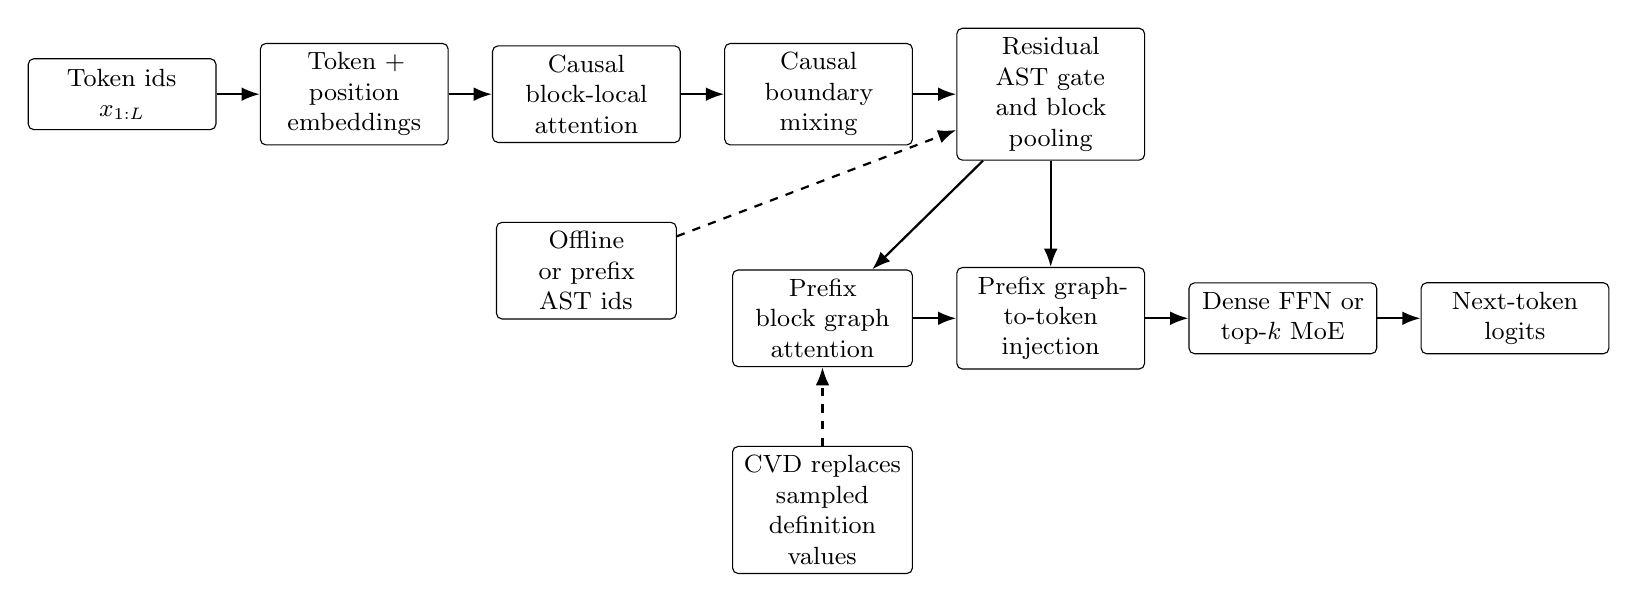
\begin{tikzpicture}[
    node distance=0.75cm and 0.55cm,
    box/.style={draw, rounded corners=2pt, align=center, minimum height=0.9cm,
      text width=2.15cm, font=\small},
    smallbox/.style={draw, rounded corners=2pt, align=center, minimum height=0.8cm,
      text width=2.05cm, font=\small},
    arrow/.style={-Latex, thick},
    dashedarrow/.style={-Latex, thick, dashed}
  ]
    \node[box] (tokens) {Token ids\\$x_{1:L}$};
    \node[box, right=of tokens] (embed) {Token + position\\embeddings};
    \node[box, right=of embed] (local) {Causal block-local\\attention};
    \node[box, right=of local] (boundary) {Causal boundary\\mixing};
    \node[box, right=of boundary] (pool) {Residual AST gate\\and block pooling};
    \node[box, below=1.35cm of pool] (inject) {Prefix graph-to-token\\injection};
    \node[box, right=of inject] (moe) {Dense FFN or\\top-$k$ MoE};
    \node[box, right=of moe] (logits) {Next-token\\logits};

    \node[smallbox, below=1.0cm of local] (ast) {Offline or prefix\\AST ids};
    \node[smallbox, left=of inject] (graph) {Prefix block graph\\attention};
    \node[smallbox, below=1.0cm of graph] (cvd) {CVD replaces sampled\\definition values};

    \draw[arrow] (tokens) -- (embed);
    \draw[arrow] (embed) -- (local);
    \draw[arrow] (local) -- (boundary);
    \draw[arrow] (boundary) -- (pool);
    \draw[arrow] (pool) -- (inject);
    \draw[arrow] (inject) -- (moe);
    \draw[arrow] (moe) -- (logits);
    \draw[dashedarrow] (ast) -- (pool);
    \draw[arrow] (pool) -- (graph);
    \draw[arrow] (graph) -- (inject);
    \draw[dashedarrow] (cvd) -- (graph);
  \end{tikzpicture}%
  }
  \caption{One CSMT-GNN layer.  Solid arrows are differentiable model paths;
  dashed arrows are structural side inputs or training-time regularization.
  CVD is applied only during training.}
  \label{fig:architecture}
\end{figure}

\subsection{Inputs, Offline AST Features, and Prefix Inference Features}

Let a token sequence be $x_{1:L}$ and let $B$ be the block size.  The sequence is
padded to $M=\lceil L/B\rceil$ blocks.  The offline preprocessor parses each
source file and writes three compact arrays:
\[
  A \in \mathbb{N}^{M \times B}, \qquad
  r \in \{0,1\}^{M}, \qquad
  u \in \{0,1\}^{L},
\]
where $A_{m,b}$ is an AST node-type id for token $b$ in block $m$, and $r_m$
marks whether block $m$ contains a variable-definition event.  The token mask
$u_t$ marks definition tokens before they are reduced to block eligibility for
CVD.  During training,
the model owns a shared embedding table $E_{\mathrm{ast}}$ and computes
$e_{m,b}=E_{\mathrm{ast}}(A_{m,b})$.  This is a deliberate correction of the
earlier prototype, which materialized random AST embeddings offline and therefore
made the syntax channel non-trainable.

When a HuggingFace fast tokenizer is provided, the preprocessor uses its offset
mapping so AST spans follow the same tokenization as the language-model tokens.
Without that tokenizer, the preprocessor falls back to Python lexical tokens and
marks the artifact accordingly; I treat that mode as a debugging path, not as a
claim of BPE-level alignment.  For offline training artifacts, the reference
preprocessor now defaults to a complete-file parse, because this gives the
cleanest AST type ids and the most reliable definition masks.  The token-level
definition mask is built from Python binding spans when the built-in parser can
parse the file; tree-sitter remains the source of AST type ids and a best-effort
fallback for incomplete code.  Prefix and per-token prefix parsing remain
explicit modes for leakage studies and generation-time feature construction,
not the default training path.

Autoregressive inference cannot assume a complete, syntactically valid file.
The reference code therefore includes a prefix feature builder that reparses the
current generated prefix, relies on tree-sitter recovery when possible, and
falls back to lexical ids when the prefix is too broken to yield a useful AST
node.  At inference time, a saved AST vocabulary is frozen: unseen node types map
to \texttt{<UNKNOWN>} rather than creating embedding ids that were never trained.
The script reports the unknown-token rate alongside latency.  This does not make
inference free.  It turns AST availability into an explicit systems question:
measure parser latency, recovery quality, vocabulary fallback, and the
degradation from offline features to prefix features.  I do not claim that this
cost is solved by the architecture.

\subsection{Block-Local Transformer Computation}

Token embeddings and positional embeddings form $H^0\in\mathbb{R}^{M\times B
\times d}$.  Each layer first applies RMSNorm and block-local self-attention:
\[
  \tilde H_m = H_m + \mathrm{Attn}_B(\mathrm{RMSNorm}(H_m)).
\]
The attention uses compressed key-value projections:
\[
  Q = HW_Q,\quad C=HW_C,\quad K=CW_K,\quad V=CW_V,
\]
which keeps the interface close to multi-head latent attention while avoiding a
custom kernel dependency in the reference implementation.

\subsection{AST-Gated Block Pooling}

The AST side channel modulates token states before pooling.  I use a residual
gate rather than a plain sigmoid gate so the initial model does not halve the
hidden-state scale.  With
$g_{m,b}=1+\lambda\tanh(W_{\mathrm{ast}} e_{m,b})$, the gated state is
\[
  \bar H_{m,b}=\tilde H_{m,b}\odot g_{m,b}.
\]
Before pooling, an initially-zero boundary module lets the first
$w_{\mathrm{bdry}}$ tokens of block $m$ receive learned corrections from the
last token of block $m-1$.  I keep this correction one-way so the language model
does not read future tokens across a block boundary.  This is a small concession
to the fact that fixed blocks can cut through syntax.  Because the boundary
projection is initialized at zero, the initial model is exactly the no-boundary
model; training must learn whether the correction is useful.
A learned query vector $q$ scores tokens within each block:
\[
  \alpha_{m,b} =
  \mathrm{softmax}_b\left(\frac{q^\top \bar H_{m,b}}{\sqrt d}\right),\qquad
  z_m=\sum_b \alpha_{m,b}\bar H_{m,b}.
\]
The result $z_m$ is a compact block state used by graph attention.  This design
keeps AST computation proportional to $L d_{\mathrm{ast}} d$ in the unfused
reference implementation and makes the cost visible for ablation.

\subsection{Prefix Block Graph and Contextual Variable Dropout}

The block states $z_{1:M}$ are passed through a prefix-masked graph attention
layer.  It is graph-like because nodes are blocks and edges point from earlier
blocks to later blocks; it is autoregressive because node $m$ cannot attend to
$n>m$:
\[
  s_{1:M}=\mathrm{PrefixGraphAttn}(z_{1:M}).
\]
In batched training, this prefix mask is combined with a valid-block key mask,
and padded block outputs are zeroed after graph attention.  I include this
detail because padding should be outside the block graph, not merely harmless
because later token states are masked.

CVD changes only the value messages.  During training, each variable-definition
block is sampled with probability $p_{\mathrm{cvd}}$.  The current
implementation prefers token-level definition masks when available and reduces
them to block eligibility; this reduces false positives from coarse block-level
labels.  For selected blocks, the
value vector is replaced by a learned vector $v_{\mathrm{cvd}}$ before graph
attention:
\[
  V_m =
  \begin{cases}
    v_{\mathrm{cvd}}, & r_m=1 \text{ and } u_m < p_{\mathrm{cvd}},\\
    W_V z_m, & \text{otherwise}.
  \end{cases}
\]
I no longer call this a causal intervention.  The operation is a structured
dropout mechanism targeted at definition-bearing blocks.  The intended effect
is to discourage brittle reliance on one local definition token and to encourage
redundant, contextually grounded representations.

\subsection{Graph-to-Token Injection and MoE}

The graph state is injected into token states with a prefix shift, so block $m$
receives graph context from previous blocks:
\[
  c_m =
  \begin{cases}
    0, & m=1,\\
    W_c\,\mathrm{RMSNorm}(s_{m-1}), & m>1.
  \end{cases}
\]
The token-level injection is gated:
\[
  H'_{m,b}=\bar H_{m,b} + W_o\left(\sigma(W_g\bar H_{m,b})\odot c_m\right).
\]
Finally, the layer applies a residual top-$k$ MoE feed-forward module.  The
reference code sorts token-expert assignments into contiguous expert batches,
which avoids the earlier per-token dynamic dispatch pattern and is a reasonable
fallback when vendor grouped GEMM kernels are not available.  The implementation
also tracks a router load-balancing loss and a router z-loss; for production
training, a grouped-GEMM expert kernel remains the right target.

\section{Implementation and Development Workflow}

\subsection{Reference Code}

My cleaned implementation is organized around small, auditable entry points:
\begin{itemize}
  \item \texttt{ast\_preprocessor.py} emits AST ids, block masks, token-level
  definition masks, and an AST vocabulary.
  \item \texttt{inference\_ast.py} builds approximate AST ids from incomplete
  generation prefixes.
  \item \texttt{diagnostics.py} creates small shadowing, long-range import, and
  guarded-attribute cases for cheap pipeline checks.
  \item The structural-probe script measures whether those diagnostic cases
  actually contain definition-use and cross-block structure.
  \item The CVD audit script records how often variable-targeted and random CVD
  sample eligible blocks.  This accounting is opt-in because it synchronizes
  device tensors for human-readable counts; the default training path samples
  masks without asking Python whether any block was selected.
  \item \texttt{transformer\_baseline.py} implements a separate token-only
  causal Transformer, including a rough parameter-neighbor control used by the
  tiny diagnostics.  It shares the same fail-fast token-id and length checks as
  the CSMT path, so baseline runs do not silently repair malformed inputs.
  \item \texttt{csmt\_gnn.py} contains the reusable architecture, and
  \texttt{train.py} supports single-process and \texttt{torchrun} training over
  paired token and AST NumPy files.  Input id range scans are enabled by
  default for fail-fast debugging, but can be disabled after the NumPy pipeline
  is validated; dtype, shape, and length checks remain active.  The trainer also
  trims AST ids and definition masks to the next-token model-input prefix before
  each forward pass, so complete-sample side inputs are not handed to a shorter
  prediction prefix.
  \item \texttt{scripts/validate\_data\_pipeline.py} is the NumPy preflight
  check for that validated-pipeline fast path: it scans token ids, AST ids,
  block shapes, masks, and usable lengths before training.
  \item \texttt{scripts/diagnostic\_poc\_train.py} trains an ablation matrix on
  the diagnostic cases when PyTorch is available.  It now trims AST ids and
  definition masks to the same next-token prefix before each CSMT forward pass
  and records a \texttt{prefix\_feature\_audit} field in its JSON output.
\end{itemize}
I treat the diagnostic output as a plumbing and falsification check, not as a
benchmark.

\subsection{Ablation-Ready Components}

The reference model exposes each contested mechanism as a real configuration
switch rather than a rhetorical promise.  \texttt{use\_ast\_gate} removes the AST
embedding table and AST projection from the model.  \texttt{use\_block\_graph}
removes the prefix graph and graph-to-token injection.  \texttt{use\_cvd}
removes the CVD replacement parameter and sampling path.  \texttt{use\_boundary}
removes the causal boundary mixer.  \texttt{use\_moe} replaces the routed MoE
with a dense SwiGLU-style feed-forward module, so the no-MoE ablation still has
feed-forward capacity.  The CVD sampler also supports
\texttt{cvd\_scope=variable} and \texttt{cvd\_scope=random}, which makes the
ordinary-noise control explicit.  These switches matter because I cannot ask a
reader to trust an architecture whose main objections cannot be isolated.
I also keep the Transformer baselines outside this switch system.  The
\texttt{transformer\_baseline} variant is a separate causal Transformer with no
AST, block graph, boundary mixer, or CVD path.  The
\texttt{transformer\_matched} variant widens the Transformer feed-forward layer
to be a rough parameter neighbor of the tiny CSMT variants.  It is not a perfect
matched study, but it is a stronger first control than comparing CSMT only
against its own disabled configurations.

\subsection{Development Audit}

The author workflow described in the introduction leaves a concrete audit trail.
The early prototype was useful because it made the architecture runnable, but it
also exposed failure modes that would have made the work indefensible if kept:
causal terminology that the computation did not earn, repeated operation guides,
a block-size-specific softmax path, random offline AST embeddings, distorted CVD
sampling, and a Python-loop expert path that would collapse throughput when
specialized kernels were unavailable.

The current reference implementation is the result of removing those weaknesses
rather than polishing their names.  I renamed the unsupported do-intervention
framing to CVD, moved AST handling to tokenizer-aligned ids with trainable
embeddings, removed the brittle fused-kernel path from the reference
implementation, added prefix inference features, corrected batch and padding
semantics, added Transformer controls, and made the release package inspectable.
This is why I treat the development process as part of the contribution.  I am
not presenting multi-LLM coding as a substitute for authorship; I am presenting
it as a way for an independent researcher to reach a testable artifact faster,
provided the final work is audited, renamed where necessary, and stripped of
claims the implementation cannot support.  The artifact is not only a proposed
architecture, but also a record of which claims survived audit and which ones
had to be deleted.

\begin{table}[t]
  \centering
  \caption{Problems in the original prototype and their corresponding fixes.}
  \label{tab:fixes}
  \small
  \begin{tabularx}{\textwidth}{@{}lYY@{}}
    \toprule
    Area & Original risk & Current fix \\
    \midrule
    AST features & Offline random embeddings & Offline ids, trainable shared embedding \\
    Token offsets & Lexical/BPE mismatch risk & Optional tokenizer offset mapping \\
    Causal claim & Mask framed as do-calculus & Renamed and scoped as CVD regularization \\
    Fused softmax & Hard-coded four chunks of 16 & Reference path uses dynamic block shape \\
    CVD sampling & Forced one mask per eligible sample & Bernoulli sampling with true zero-mask cases \\
    CVD auditing & Per-step count sync in training path & Audit counts are opt-in; default sampling is synchronization-free \\
    Padding in graph path & Padded blocks could remain graph nodes & Valid-block attention mask and zeroed padded block outputs \\
    Trainer side inputs & Full-sample AST features during next-token prediction & Prefix-trimmed AST ids and masks before forward pass \\
    Inference AST & Assumed complete-file parse & Prefix parser with lexical fallback \\
    Block boundaries & Hard cuts through syntax & Initially-zero causal boundary mixing before pooling \\
    MoE fallback & Token-wise dynamic dispatch & Sorted top-$k$ contiguous expert batches \\
    Ablations & Only baseline/full comparison & Component switches plus random-dropout control \\
    Documentation & Repeated guides inside code & Separate source files and paper artifact \\
    Training checks & Per-step id range scans always on & Default fail-fast checks with an explicit validated-pipeline fast path \\
    \bottomrule
  \end{tabularx}
\end{table}

My choice to remove the hand-written Triton F1 kernel from the reference path is
intentional.  The earlier kernel assumed $B=64$ in its second-stage softmax.  A
production kernel should either be generated for supported block sizes or use a
shape-parametric reduction.  Until that exists, the correct reference
implementation is more valuable than a fast path with undefined behavior at
other block sizes.

\section{Theoretical Checks and Complexity}
\label{sec:theory}

Algebra cannot replace training evidence, but it can rule out basic failure
modes before scaling: future leakage in the block graph, unbounded changes from
the AST gate at initialization, unsupported memory claims, and a CVD story with
no objective behind it.  These checks are deliberately modest; their purpose is
to make the mechanism auditable before any performance claim is attached to it.
Detailed proofs are collected in Appendix~\ref{app:proofs}, so the main text can
stay focused on what each statement means for the architecture.

\begin{proposition}[Prefix visibility]
\label{prop:prefix}
Assume each block-local attention operator uses a causal mask, the block graph
attends only from block $m$ to valid blocks $n\le m$, and padded block outputs
are not injected into real token states.  If the AST ids for token $t$ are
computed from a source prefix ending no later than $t$, then the hidden state
used to predict token $t+1$ is a function only of tokens and AST spans in the
prefix $x_{1:t}$.
\end{proposition}


The default offline training preprocessor uses complete-file parsing for
cleaner syntax labels and definition masks.  Proposition~\ref{prop:prefix} is
therefore not a claim that every training artifact is prefix-only.  It is the
contract for generation-time features and for experiments that require strict
prefix preprocessing.  When training uses complete-file features and inference
uses prefix features, the relevant question is the measured drift between those
two side inputs, which I define in Proposition~\ref{prop:prefix-metrics}.

\begin{proposition}[Causal boundary mixing]
\label{prop:boundary}
Let the boundary module update only the first $w_{\mathrm{bdry}}$ token states
of block $m$ using a learned function of the last token state of block $m-1$:
\[
  \hat H_{m,b}
  =
  \tilde H_{m,b}
  + \mathbf{1}[b\le w_{\mathrm{bdry}}]\,
    \gamma\,P_b(\tilde H_{m-1,B}),\qquad m>1 .
\]
If $\tilde H_{m-1,B}$ is causal with respect to tokens up to the end of block
$m-1$, then $\hat H_{m,b}$ is causal with respect to tokens up to position
$(m-1)B+b$.  In particular, the boundary module cannot transmit information
from block $m$ or any later block into block $m-1$.
\end{proposition}


\begin{proposition}[Attention-edge count]
\label{prop:edges}
For $L=MB$ tokens, full causal token attention uses
$L(L+1)/2$ token-token edges.  CSMT-GNN uses
$M B(B+1)/2$ block-local token edges plus $M(M+1)/2$ block graph edges.  The edge
ratio is
\[
  \rho(B,M)=
  \frac{M B(B+1)+M(M+1)}{M B(MB+1)}.
\]
For fixed $B$ and large $M$, the graph term contributes an asymptotic ratio
$1/B^2$ and the local term contributes $O(1/M)$.  Thus a fixed block size gives
a constant-factor reduction in the quadratic graph term, not a change of
asymptotic order.  If $B$ is allowed to scale with $L$, choosing
$B=\Theta(L^{1/3})$ balances the two terms and gives $O(L^{4/3})$ edges.
\end{proposition}


This edge count does not say the implementation is automatically faster.  It
says where the architecture moves communication: from dense token-token
interactions to short token windows plus a smaller graph.  For hidden size
$d$, the leading attention arithmetic is
$O(MB^2d+M^2d)=O(LBd+L^2d/B^2)$.  The AST gate adds
$O(Ld_{\mathrm{ast}}d)$ projection work and the MoE adds routed expert work.
Those extra terms are exactly why the AST channel must later pass an efficiency
ablation.

\begin{corollary}[Block-size trade-off]
\label{cor:block-size}
If the dominant structured-attention cost is approximated by
$T(B)=aLB+bL^2/B^2$ for positive constants $a$ and $b$, then the continuous
minimizer is
\[
  B^\star = \left(\frac{2bL}{a}\right)^{1/3}.
\]
Thus no single fixed block size is theoretically privileged across all sequence
lengths and hardware constants.
\end{corollary}


This corollary is why I treat block size as an experimental variable rather
than a magic number.  The reference code supports arbitrary positive block sizes
within shape constraints, and the paper should report a sweep before defending a
particular $B$.
The repository includes \texttt{scripts/architecture\_cost\_table.py}, which
turns this accounting into a small JSON table.  For example, at
$L=2048,B=64$, dense causal attention has 2,098,176 causal token edges, while
block-local causal attention plus the causal block graph has 67,088 counted
edges in this simplified model.  That number is not a runtime benchmark, but it
does make the intended communication trade-off concrete.

\begin{proposition}[Long-range summary path]
\label{prop:path}
For any two block indices $i<j$, one CSMT-GNN layer contains a differentiable
computational path from the pooled state $z_i$ to every injected token state
$H'_{j,b}$ in block $j$.  A block-local Transformer layer without cross-block
communication has no such one-layer path.
\end{proposition}


This is the structural reason I added the graph.  It does not force the model to
use a distant block, but it makes the route available without asking token-level
attention to pay the full $L^2$ price.

\begin{proposition}[Residual AST gate stability]
\label{prop:gate}
Let $g_{m,b}=1+\lambda\tanh(W_{\mathrm{ast}}e_{m,b})$ with elementwise
multiplication $\bar H_{m,b}=H_{m,b}\odot g_{m,b}$.  If $0\le\lambda<1$, then
each coordinate of the gate lies in $[1-\lambda,1+\lambda]$, and
\[
  (1-\lambda)\|H_{m,b}\|_2
  \le \|\bar H_{m,b}\|_2
  \le (1+\lambda)\|H_{m,b}\|_2 .
\]
\end{proposition}


This is why I use a residual gate instead of a sigmoid gate.  A sigmoid starts
near $1/2$ and immediately rescales the hidden stream.  The residual gate starts
near identity and lets the model learn how much syntax should matter.

\begin{proposition}[AST gate containment and cost boundary]
\label{prop:ast-cost}
Let $\mathcal{F}_0$ be the model family obtained by removing AST-gated pooling,
and let $\mathcal{F}_{\mathrm{ast}}$ be the same family with the residual gate
from Proposition~\ref{prop:gate}.  Because $W_{\mathrm{ast}}=0$ gives
$g_{m,b}=1$, $\mathcal{F}_0\subseteq\mathcal{F}_{\mathrm{ast}}$.  Therefore the
minimum unregularized empirical risk over $\mathcal{F}_{\mathrm{ast}}$ is no
larger than the minimum over $\mathcal{F}_0$.  If deployment is judged by
$J(f)=R(f)+\eta C(f)$, where $R$ is task risk, $C$ is compute cost, and
$\eta>0$, then the AST side channel improves the deployment objective only when
\[
  R(f_0^\star)-R(f_{\mathrm{ast}}^\star)
  >
  \eta\big(C(f_{\mathrm{ast}}^\star)-C(f_0^\star)\big).
\]
\end{proposition}


This proposition is deliberately plain.  It does not say optimization will find
the better member of the larger family, and it does not say the added structure
will generalize.  It says the AST channel is not justified by expressivity
alone.  The extra projection work and preprocessing complexity must buy enough
risk reduction to cross the displayed threshold.

\begin{proposition}[Prefix AST degradation metrics]
\label{prop:prefix-metrics}
For a finished file, let $A^{\mathrm{full}}_t$ be the AST type id assigned to
token $t$ by a complete-file parse, and let $A^{\mathrm{pref}}_t$ be the id
assigned when parsing only the generation prefix ending at $t$.  Let
$F_t\in\{0,1\}$ indicate that the prefix extractor fell back to a lexical token
type, and let $U_t\in\{0,1\}$ indicate that the frozen training vocabulary maps
the extracted type to \texttt{<UNKNOWN>}.  Three quantities summarize the
inference AST path:
\[
  r_{\mathrm{fb}}=\frac{1}{L}\sum_{t=1}^L F_t,\qquad
  r_{\mathrm{unk}}=\frac{1}{L}\sum_{t=1}^L U_t,\qquad
  d_{\mathrm{pref}}=\frac{1}{L}\sum_{t=1}^L
  \mathbf{1}\!\left[A^{\mathrm{pref}}_t\ne A^{\mathrm{full}}_t\right].
\]
If any of these rates is large, the AST side channel at inference time is not
the same side channel used in offline training and must be cached, throttled,
regularized against, or removed.
\end{proposition}


\begin{proposition}[CVD as stochastic smoothing]
\label{prop:cvd}
For an example with eligible definition blocks $\mathcal{D}$, let
$\xi_m\sim\mathrm{Bernoulli}(p_{\mathrm{cvd}})$ independently for
$m\in\mathcal{D}$.  Let $f_\theta(x,A,\xi)$ denote the CSMT-GNN prediction after
replacing value messages of sampled blocks by $v_{\mathrm{cvd}}$.  Training with
CVD minimizes an unbiased Monte Carlo estimate of
\[
  \mathcal{L}_{\mathrm{cvd}}(\theta)
  =
  \mathbb{E}_{(x,y)}
  \mathbb{E}_{\xi}
  \left[\ell(f_\theta(x,A,\xi),y)\right].
\]
Moreover, a given eligible block is masked at least once in $T$ independent
presentations with probability $1-(1-p_{\mathrm{cvd}})^T$.
\end{proposition}


\begin{corollary}[Gradient exposure of the CVD replacement vector]
\label{cor:cvd-gradient}
The replacement vector $v_{\mathrm{cvd}}$ receives gradient support only through
positions whose value messages are sampled for replacement.  If an example has
$D$ eligible blocks, at least one such position is sampled with probability
$1-(1-p_{\mathrm{cvd}})^D$ on a single presentation and probability
$1-(1-p_{\mathrm{cvd}})^{DT}$ across $T$ independent presentations.
\end{corollary}


This proposition is the right mathematical description of CVD.  It is a
structured stochastic smoothing objective over definition-bearing block
messages.  It is not a do-calculus intervention, and it gives no guarantee that
structural hallucination will fall.  What it does guarantee is that the training
objective explicitly includes predictions under definition-message replacement,
with a tunable exposure probability.  It also explains why the old dummy-gradient
trick was the wrong abstraction: the right statement is probabilistic gradient
support, not guaranteed learning signal on every step.  The reference trainer
therefore leaves the optional L2 penalty on $v_{\mathrm{cvd}}$ disabled by
default; turning it on is a practical stabilization choice, not part of the CVD
objective above.

\begin{proposition}[Bounded CVD value perturbation]
\label{prop:cvd-bound}
Consider one graph-attention head at query block $q$, with attention weights
$a_{qm}\ge 0$ and $\sum_m a_{qm}=1$.  Let $\mathcal{S}$ be the sampled CVD mask.
If unmasked values and the replacement vector satisfy
$\|V_m\|_2\le R$ and $\|v_{\mathrm{cvd}}\|_2\le R$, then replacing sampled values
changes the head output by at most
\[
  2R \sum_{m\in\mathcal{S}} a_{qm}.
\]
\end{proposition}


This bound is another reason I prefer the CVD framing.  The operation is a
controlled value-message perturbation whose size depends on attention mass over
masked definition blocks; it is not a literal deletion of a semantic variable.

\section{Evaluation Protocol}

I keep the evaluation plan separate from measured results.  The theory above is
a filter for internal consistency; it is not a substitute for empirical
validation.  Before treating CSMT-GNN as a competitive code model, I would start
with five uncomfortable questions that can break the mechanism quickly.

\begin{table}[t]
  \centering
  \caption{Staged falsification plan.  The point is not to make a small run look
  like a benchmark, but to decide what should be tested before scaling the
  architecture.}
  \label{tab:stages}
  \begin{tabularx}{\linewidth}{P{0.14\linewidth}P{0.28\linewidth}YY}
    \toprule
    Stage & Run & Pass signal & Stop signal \\
    \midrule
    0 & Static checks, prefix AST latency, fallback/unknown rates, shape tests. &
    No future-leakage path is detected; AST feature construction is measurable. &
    Prefix parsing dominates decoding or produces mostly fallback/unknown ids. \\
    1 & Tiny diagnostic training on shadowing, imports, guarded attributes, and
    class ownership. &
    AST/CVD variants improve dependency-sensitive loss or preservation over
    token-only, random-dropout, and Transformer controls. &
    The full model fails to beat the cheap controls on diagnostics, or the
    parameter-neighbor Transformer explains the gain. \\
    2 & Small parameter-matched ablations on Python code. &
    AST graph gains survive throughput and memory accounting. &
    Gains are smaller than the cost of preprocessing and graph computation. \\
    3 & Larger code model attempt with fused kernels or grouped GEMM. &
    Structural gains persist when the reference bottlenecks are replaced by
    production kernels. &
    The architecture only works in the toy setting or one hand-picked block
    size. \\
    \bottomrule
  \end{tabularx}
\end{table}

\paragraph{Can prefix AST features survive generation?}
The first inference test measures whether the prefix AST path is usable during
autoregressive decoding.  Feed incomplete prefixes such as
\texttt{def f(x}:, half-written class bodies, and open comprehensions into the
prefix feature builder.  The repository exposes this as a direct timing check
through \texttt{inference\_ast.py --repeat N} and as a full-vs-prefix
degradation check through \texttt{scripts/prefix\_ast\_degradation.py}.  Report
parse success, fallback rate, unknown-token rate under the frozen training
vocabulary, feature latency per generated token, and the divergence between
prefix AST ids and complete-file AST ids after the code is finished.  If this latency
dominates decoding, AST conditioning should be cached, throttled to block
boundaries, or removed.

\paragraph{Does AST help enough to pay for itself?}
The second ablation is deliberately harsh: train parameter-matched models with
and without AST-gated pooling, and include a plain Transformer with comparable
parameter count and training budget.  Report
tokens/sec, memory use, validation loss, HumanEval/MBPP pass@1, and AST-sensitive
diagnostics.  The decision rule should include efficiency: a small accuracy gain
with large throughput loss is not a win for practical code modeling.

\paragraph{How sensitive is the model to block size?}
The third ablation sweeps $B\in\{32,64,128\}$ and records throughput, memory,
validation loss, and errors on examples where definitions or syntactic spans
cross block boundaries.  Compare boundary mixing on and off.  A method that only
works for one hand-picked block size is not robust enough to defend.

\paragraph{Does CVD reduce structural hallucination?}
The fourth ablation asks whether CVD is doing anything more useful than ordinary
noise.  Construct tests where the correct answer depends on definitions separated from
uses.  Examples include variable shadowing, renamed parameters, branch-guarded
attributes, long-range imports, and class-method ownership.  Compare no CVD,
random block dropout, and variable-definition CVD.  The key metric is not just
surface match but whether generated code preserves the relevant dependency.

\paragraph{Does the block graph carry useful state?}
The fifth ablation is about the graph itself.  Ablate graph attention, prefix
injection, and graph depth.  Inspect whether
failures cluster in long files and whether the graph helps more as definition
and use distance increases.  This is where the architecture should earn its
extra complexity.

\paragraph{Minimum proof-of-concept before scale.}
Before any large training run, I should run a deliberately small diagnostic:
create synthetic Python files for variable shadowing, long-range imports, and
guarded attributes, train tiny parameter-matched models for a fixed number of
steps, and report whether AST/CVD changes the masked-token loss or dependency
preservation on those diagnostics.  The repository includes a diagnostic data
generator for this purpose.  Passing this test would not prove the architecture;
failing it would be a useful early falsification.

\begin{table}[t]
  \centering
  \caption{Recommended ablation matrix.  The same names are used by the tiny
  diagnostic script before any larger parameter-matched run.}
  \label{tab:ablations}
  \begin{tabular}{lllll}
    \toprule
    Variant & AST gate & Block graph & CVD & FFN path \\
    \midrule
    \texttt{transformer\_baseline} & No & No & No & Transformer FFN \\
    \texttt{transformer\_matched} & No & No & No & Wider Transformer FFN \\
    \texttt{token\_baseline} & No & No & No & Dense \\
    \texttt{boundary\_only} & No & No & No & Dense \\
    \texttt{ast\_only} & Yes & No & No & Dense \\
    \texttt{graph\_only} & No & Yes & No & Dense \\
    \texttt{ast\_graph} & Yes & Yes & No & Dense \\
    \texttt{random\_dropout\_control} & Yes & Yes & Random blocks & Dense \\
    \texttt{variable\_cvd} & Yes & Yes & Definition blocks & Dense \\
    \texttt{full\_moe} & Yes & Yes & Definition blocks & MoE \\
    \bottomrule
  \end{tabular}
\end{table}

\section{Limitations}

The first limitation is the validation level.  The current artifact is a
corrected prototype and paper design, not a fully trained model with large-scale
empirical claims.  I therefore separate mechanism checks from performance
claims: prefix dependence, edge-count accounting, gate stability, and the
stochastic objective induced by CVD help make the architecture inspectable, but
they do not prove that CSMT-GNN beats established code LLMs.  The release should
be read as a falsifiable design artifact rather than a leaderboard result.

The second limitation is the causal framing.  CVD was motivated by
counterfactual thinking, but it is not an identified SCM intervention.  If I or
someone else wants to make a causal claim later, the work must specify variables,
structural equations, intervention targets, and assumptions connecting code
syntax to program behavior.  I deliberately avoid that stronger claim here
because the implementation does not earn it.

The third limitation is AST coverage.  The current preprocessor focuses on
Python.  Extending to multilingual code requires language-specific parsers,
stable vocabularies, and careful token alignment with the tokenizer used for
training.  Tree-sitter can help, but the engineering is not automatic.

The fourth limitation is inference-time parsing.  Training can use offline AST
features, while generation only has a partial prefix that may be syntactically
invalid.  I added a prefix AST builder with parser recovery and lexical
fallback, but this is not a proof that the latency is acceptable.  A real
deployment must measure how often prefix features differ from complete-file
features and whether caching at block boundaries is enough.

Finally, the architecture may simply be too expensive or too sensitive to the
block size.  I added an initially-zero boundary mixing module to reduce hard
cuts through syntax, but the right block size still has to be measured.  The
design should survive cost-sensitive ablation before it is treated as a
deployment candidate.  If the AST gate and block graph do not improve downstream
reliability enough to justify their cost, the right conclusion is to simplify
the model.

\section{Broader Impact}

Better code models can make programming more accessible and can reduce routine
engineering labor.  They can also generate insecure code faster, help automate
malicious scripting, or give users unwarranted confidence in plausible but wrong
programs.  CSMT-GNN is aimed at reducing structural mistakes in code generation,
but the same capability could improve both benign and harmful automation.  Any
release of trained checkpoints should include standard code-safety evaluation,
license-aware data handling, and clear warnings that generated code requires
review and testing.

\section{Conclusion}

CSMT-GNN is my attempt to make a code language model carry a little more of the
program's structure without giving up token-level generation.  The revised
implementation is less grand than my first notes, and I think that is a good
thing.  It keeps the parts I still believe are worth testing--tokenizer-aligned
AST ids, trainable syntax embeddings, prefix-masked block graph attention, and
CVD over definition-bearing blocks--while removing claims and code paths that
did not survive inspection.  The result is narrower, but it is also more
durable: a structure-aware code-model design, a reference implementation, and a
diagnostic harness whose assumptions are visible enough to inspect and challenge.

\bibliographystyle{plainnat}
\bibliography{references}

\appendix

\section{Proofs for the Theoretical Checks}
\label{app:proofs}

\begin{proof}[Proof of Proposition~\ref{prop:prefix}]
Inside a block, causal self-attention prevents position $b$ from reading
positions greater than $b$.  The block graph receives pooled summaries from
valid blocks with index at most the current block; with the injection shift used
in Section 3.5, block $m$ receives only graph state from valid blocks $<m$.
Padded block outputs are zeroed and are not injected into real token states.
Therefore no later block can affect the current token state.  The remaining possible leakage
source is preprocessing: if AST ids are built from the complete file, a token can
receive node information created by later syntax.  The per-token prefix mode
removes that source by construction, because the parser input ends at the token
boundary.  Composing these three facts gives the prefix dependence claim.
\end{proof}

\begin{proof}[Proof of Proposition~\ref{prop:boundary}]
The update to block $m$ depends on two quantities: the current token state
$\tilde H_{m,b}$ and the previous-block tail $\tilde H_{m-1,B}$.  By causal
block attention, $\tilde H_{m,b}$ depends only on tokens within block $m$ up to
position $b$, and by the premise $\tilde H_{m-1,B}$ depends only on tokens up to
the end of block $m-1$.  Their sum therefore depends only on the union of those
prefixes, which is exactly the token prefix ending at $(m-1)B+b$.  The module
contains no path from block $m$ to block $m-1$, because the projection is applied
from the previous block tail to the current block head only.
\end{proof}

\begin{proof}[Proof of Proposition~\ref{prop:edges}]
The full causal mask is triangular over $L$ positions.  Each of the $M$ local
blocks contributes $B(B+1)/2$ causal edges.  The prefix block graph is triangular
over $M$ block nodes, contributing $M(M+1)/2$ edges.  Dividing the structured
edge count by the full edge count gives the displayed ratio.  Substituting
$M=L/B$ gives $O(LB)+O(L^2/B^2)$ edges.  The two terms balance when
$LB=L^2/B^2$, i.e. $B=\Theta(L^{1/3})$, yielding $O(L^{4/3})$ edges.
\end{proof}

\begin{proof}[Proof of Corollary~\ref{cor:block-size}]
Differentiate $T(B)$ with respect to $B$:
$T'(B)=aL-2bL^2/B^3$.  Setting $T'(B)=0$ gives
$B^3=2bL/a$.  The second derivative $6bL^2/B^4$ is positive, so this critical
point is a minimum.
\end{proof}

\begin{proof}[Proof of Proposition~\ref{prop:path}]
In the prefix block graph, state $s_{j-1}$ is computed by attention over block
states $z_1,\ldots,z_{j-1}$, which includes $z_i$.  The graph-to-token injection
then maps $s_{j-1}$ through $W_c$, gates it with a token-dependent gate, and adds
the result to every token in block $j$.  This gives the path
$z_i\rightarrow s_{j-1}\rightarrow c_j\rightarrow H'_{j,b}$.  In a layer whose
attention is restricted to tokens inside each block, the output of block $j$ is
a function only of block $j$'s input tokens, so no one-layer path from block
$i<j$ exists.
\end{proof}

\begin{proof}[Proof of Proposition~\ref{prop:gate}]
For every coordinate, $\tanh(\cdot)\in[-1,1]$, so
$g_i\in[1-\lambda,1+\lambda]$.  Since $g_i$ is nonnegative when
$\lambda<1$, the squared norm of the gated vector is bounded between
$(1-\lambda)^2\sum_i H_i^2$ and $(1+\lambda)^2\sum_i H_i^2$.  Taking square
roots proves the claim.
\end{proof}

\begin{proof}[Proof of Proposition~\ref{prop:ast-cost}]
Setting $W_{\mathrm{ast}}=0$ makes the residual gate exactly one in every
coordinate, so every no-AST model is represented inside the AST-gated family.
Taking an infimum of the same empirical loss over a superset cannot increase
the optimum.  The deployment inequality follows by expanding
$J(f_{\mathrm{ast}}^\star)<J(f_0^\star)$ and moving the compute term to the
right-hand side.
\end{proof}

\begin{proof}[Proof of Proposition~\ref{prop:prefix-metrics}]
The three rates are empirical averages over token-level Bernoulli indicators.
They are therefore in $[0,1]$ and measure distinct failure modes: parser
recovery or lexical fallback, vocabulary mismatch, and disagreement with a
complete-file parse after the file is known.  A model trained on complete-file
or low-fallback AST ids receives a shifted side input when these rates grow.
The proposition is a measurement contract rather than a performance guarantee:
it identifies when inference-time AST conditioning has drifted from the training
artifact.
\end{proof}

\begin{proof}[Proof of Proposition~\ref{prop:cvd}]
The implementation samples $\xi$ and evaluates the loss for that sampled masked
graph.  The stochastic gradient is therefore the gradient of one draw from the
inner expectation.  Under the usual interchange conditions used for stochastic
gradient training, its expectation equals
$\nabla_\theta \mathcal{L}_{\mathrm{cvd}}(\theta)$.  The second statement is the
complement of never sampling the block in $T$ independent Bernoulli trials.
\end{proof}

\begin{proof}[Proof of Corollary~\ref{cor:cvd-gradient}]
The vector $v_{\mathrm{cvd}}$ is used only when some Bernoulli mask is one.  The
probability that all $D$ masks are zero is $(1-p_{\mathrm{cvd}})^D$, and the
same complement argument over $DT$ independent trials gives the multi-pass
statement.
\end{proof}

\begin{proof}[Proof of Proposition~\ref{prop:cvd-bound}]
The unmasked head output is $o_q=\sum_m a_{qm}V_m$ and the masked output is
$\tilde o_q=\sum_{m\notin\mathcal{S}}a_{qm}V_m+
\sum_{m\in\mathcal{S}}a_{qm}v_{\mathrm{cvd}}$.  Their difference is
$\tilde o_q-o_q=\sum_{m\in\mathcal{S}}a_{qm}(v_{\mathrm{cvd}}-V_m)$.  By the
triangle inequality and the norm bounds,
$\|\tilde o_q-o_q\|_2\le\sum_{m\in\mathcal{S}}a_{qm}
(\|v_{\mathrm{cvd}}\|_2+\|V_m\|_2)\le 2R\sum_{m\in\mathcal{S}}a_{qm}$.
\end{proof}

\section{Reproducibility Notes}

The public reproducibility repository is available at
\href{https://github.com/ShengyaoLiang/csmt-gnn}{https://github.com/ShengyaoLiang/csmt-gnn}.
The current \texttt{v0.1.1} archived release is
\href{https://doi.org/10.5281/zenodo.20844185}{https://doi.org/10.5281/zenodo.20844185};
the stable all-version Zenodo concept DOI is
\href{https://doi.org/10.5281/zenodo.20840624}{https://doi.org/10.5281/zenodo.20840624}.
I release the source package, paper source, tests, small diagnostic artifacts,
and packaging scripts so that the evidence chain can be inspected without
relying on private training data, hidden scripts, or unpublished checkpoints.

The source tree contains:
\begin{itemize}
  \item \texttt{ast\_preprocessor.py}: offline AST id and variable-mask builder.
  \item \texttt{inference\_ast.py}: prefix AST feature builder for incomplete generation prefixes.
  \item \texttt{scripts/prefix\_ast\_degradation.py}: full-vs-prefix AST drift measurement.
  \item \texttt{scripts/architecture\_cost\_table.py}: structural edge-count and block-size trade-off audit.
  \item \texttt{diagnostics.py}: tiny structural diagnostic data generator.
  \item \texttt{scripts/structural\_probe\_eval.py}: definition-use coverage check for the diagnostic cases.
  \item \texttt{scripts/cvd\_mask\_audit.py}: CVD eligible/sampled block audit.
  \item \texttt{scripts/validate\_data\_pipeline.py}: NumPy token/AST preflight before training fast paths.
  \item \texttt{scripts/diagnostic\_poc\_train.py}: tiny ablation sanity check.
  \item \texttt{transformer\_baseline.py}: independent token-only Transformer
  baseline for the diagnostic comparison.
  \item \texttt{scripts/build\_arxiv\_package.py}: arXiv source package builder.
  \item \texttt{csmt\_gnn.py}: model architecture.
  \item \texttt{train.py}: single-process and distributed training entry point.
  \item \texttt{requirements.txt}: minimal Python dependencies.
  \item \texttt{results/lowcompute\_validation\_summary.md}: local laptop smoke
  validation record, if included in the public code release.
\end{itemize}

A minimal debugging command is:
\begin{verbatim}
python ast_preprocessor.py \
  --source-file example.py \
  --output-dir ast_data
\end{verbatim}

For training artifacts, use tokenizer offsets.  The default is complete-file
offline parsing:
\begin{verbatim}
python ast_preprocessor.py \
  --source-file example.py \
  --output-dir ast_data \
  --tokenizer-name-or-path /path/to/tokenizer
\end{verbatim}

For strict prefix-only preprocessing studies, use the explicit slow mode:
\begin{verbatim}
python ast_preprocessor.py \
  --source-file example.py \
  --output-dir ast_data_prefix \
  --tokenizer-name-or-path /path/to/tokenizer \
  --per-token-prefix
\end{verbatim}

For prefix inference features:
\begin{verbatim}
python inference_ast.py --source-file partial_generation.py \
  --vocab-path ast_data/ast_vocab.json \
  --repeat 32
\end{verbatim}

For full-vs-prefix AST degradation:
\begin{verbatim}
python scripts/prefix_ast_degradation.py \
  --source-file example.py \
  --vocab-path ast_data/ast_vocab.json \
  --output results/prefix_ast_degradation.json
\end{verbatim}

For the structural edge-count audit:
\begin{verbatim}
python scripts/architecture_cost_table.py \
  --output results/architecture_cost_table.json
\end{verbatim}

For the smallest structural diagnostic arrays:
\begin{verbatim}
python diagnostics.py --output-dir tmp/diagnostics --block-size 8
\end{verbatim}

For structural coverage and CVD sampling audits:
\begin{verbatim}
python scripts/structural_probe_eval.py \
  --output results/structural_probe_eval.json \
  --block-size 8 --max-tokens 64

python scripts/cvd_mask_audit.py \
  --output results/cvd_mask_audit.json \
  --steps 24 --hidden-size 16 --ast-dim 8 \
  --block-size 8 --max-tokens 64
\end{verbatim}

A minimal training command, assuming paired token arrays are present, is:
\begin{verbatim}
python train.py \
  --data-path tokenized_data \
  --ast-path ast_data \
  --num-layers 12 \
  --hidden-size 768 \
  --block-size 64 \
  --max-tokens 2048 \
  --boundary-width 2
\end{verbatim}

When PyTorch is available, the local diagnostic sanity check is:
\begin{verbatim}
python scripts/diagnostic_poc_train.py --steps 12 \
  --output results/diagnostic_poc_transformer.json
\end{verbatim}

On my local laptop, I ran this diagnostic at
\texttt{hidden\_size=16}, \texttt{max\_tokens=64}, and 12 steps per variant,
plus small block-size and seed smoke sweeps.  The diagnostic now includes a pure
token-only Transformer and a rough parameter-neighbor Transformer control.  The
unit tests now pass at 39/39 after adding fail-fast checks for the Transformer
controls, incremental AST configuration checks, opt-in CVD audit coverage,
validated-pipeline input range controls, graph padding-mask coverage, trainer
prefix-trim coverage, diagnostic prefix-audit coverage, and a regression test
for token-level CVD masks on short next-token inputs.  A two-step diagnostic
run also recorded \texttt{prefix\_feature\_audit.all\_prefix\_aligned=1.0} with
an empty violation list, confirming that the diagnostic CSMT variants receive
prefix-clipped AST ids and definition masks.  The data-pipeline preflight also passed on the tiny
diagnostic arrays, checking token ids, AST ids, block shapes, masks, and usable
sequence lengths.
The structural probe found cross-block definition-use pairs in all three
diagnostic cases.  The CVD audit recorded 72 variable-eligible blocks and 112
random-control eligible blocks over 24 audited steps, with both sampling rates
near the configured 0.2.  The tiny training run showed that random CVD and
variable CVD were almost identical in final next-token loss.  I treat this
record only as a mechanism and plumbing check: it shows that the reference paths
can train on CPU and that the masks are observable, not that the architecture is
better than a baseline.

\begin{table}[t]
  \centering
  \caption{Local CPU diagnostic at seed 7, block size 8, hidden size 16, and 12
  steps per variant.  This is not a benchmark; it is a small falsification and
  plumbing check.}
  \label{tab:local_diag_main}
  \small
  \begin{tabular}{lrrrr}
    \toprule
    Variant & Params & Final loss & Eval loss & Cross-block use loss \\
    \midrule
    \texttt{transformer\_baseline} & 4688 & 3.6034 & 3.6342 & 3.6809 \\
    \texttt{transformer\_matched} & 6992 & 3.6751 & 3.5889 & 3.7469 \\
    \texttt{token\_baseline} & 4576 & 3.7727 & 3.7131 & 3.9152 \\
    \texttt{graph\_only} & 6384 & 3.7367 & 3.6630 & 3.6176 \\
    \texttt{ast\_graph} & 6960 & 3.9444 & 3.6480 & 3.5019 \\
    \texttt{variable\_cvd} & 6976 & 3.6431 & 3.5470 & 3.8563 \\
    \texttt{full\_moe} & 8160 & 3.6942 & 3.6087 & 3.2707 \\
    \bottomrule
  \end{tabular}
\end{table}

\begin{table}[t]
  \centering
  \caption{Seed 1--3 mean local diagnostic results at block size 8.  Parentheses
  show population standard deviation.  The close result between
  \texttt{transformer\_matched} and \texttt{ast\_graph} is why I do not claim a
  Transformer win or a CSMT-GNN win from this run.}
  \label{tab:local_diag_seeds}
  \small
  \begin{tabular}{lrrr}
    \toprule
    Variant & Params & Final loss & Cross-block use loss \\
    \midrule
    \texttt{transformer\_baseline} & 4688 & 3.7680 (0.0121) & 3.6739 (0.1213) \\
    \texttt{transformer\_matched} & 6992 & 3.6885 (0.0832) & 3.5243 (0.3131) \\
    \texttt{ast\_graph} & 6960 & 3.6777 (0.0955) & 3.5366 (0.2761) \\
    \texttt{variable\_cvd} & 6976 & 3.7446 (0.0514) & 3.8471 (0.2794) \\
    \texttt{full\_moe} & 8160 & 3.6761 (0.0412) & 3.7173 (0.1219) \\
    \bottomrule
  \end{tabular}
\end{table}

My reading of these numbers is cautious.  On the seed-7 run, block-graph
variants improve the cross-block use loss over the CSMT token baseline.  Across
seeds 1--3, however, the rough parameter-neighbor Transformer and
\texttt{ast\_graph} are essentially tied on mean cross-block use loss.  CVD is
also unstable in this tiny setup.  This is exactly the kind of result I wanted
the diagnostic to be able to show: the architecture is now comparable against a
real Transformer control, but it has not earned a claim that it beats
Transformer.

The arXiv source package is built with:
\begin{verbatim}
python scripts/build_arxiv_package.py
\end{verbatim}

\end{document}

